\begin{figure}[t]
\begin{center}
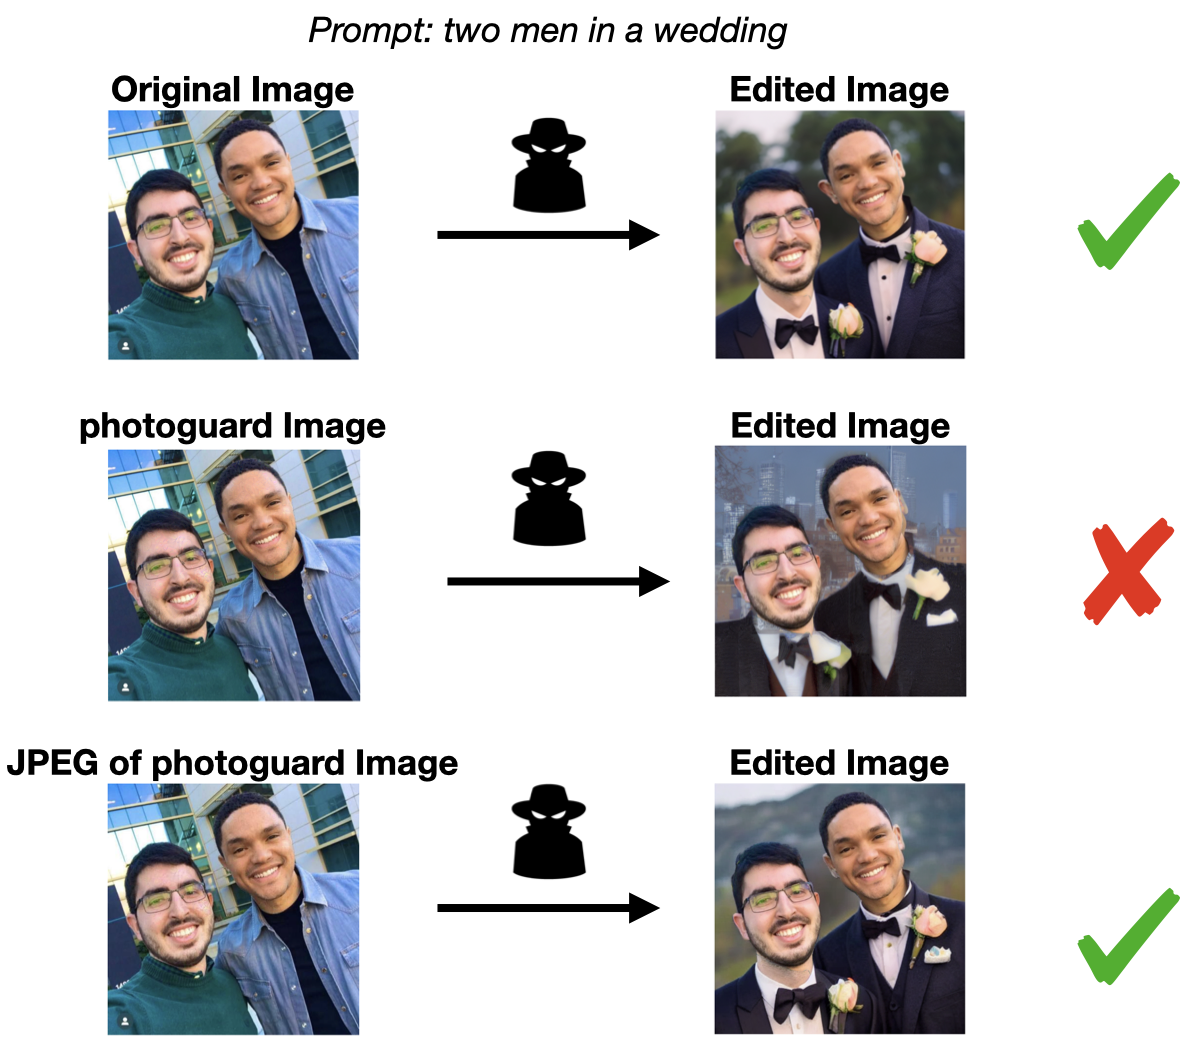
\includegraphics[width=0.67\textwidth]{images/complex-diffusion-inpaint.001.png}
\end{center}
\caption{\textbf{JPEG compression allows an adversary to edit the background of a protected image found online.} First row: Given a text prompt, an adversary can make desired edits to an input image using a diffusion model. Second row: photoguard (Diffusion attack) \citep{salman2023raising} protects the original image before an adversary can access it by adding an imperceptible perturbation. When the adversary edits the photoguard image, the background is unrealistic. Third row: By JPEG compressing the photoguard image, an adversary can edit the photoguard image while maintaining the original subjects and adding key visual features of the text prompt.}
\label{fig:inpainting-overview}
\end{figure}